\documentclass[12pt]{article}

\usepackage{graphicx}

\usepackage[margin=1in,dvips]{geometry}

\usepackage{deluxetable}

\newcommand{\commissdate}{Fall 2012}
\newcommand{\surveyproper}{Spring 2013}
\newcommand{\devauc}{De Vaucouleurs'}
\newcommand{\devprof}{exp$(-r^{1/4})$}
\newcommand{\speedupnum}{10}
\newcommand{\ncpus}{12}
\newcommand{\speedupcpu}{42.5}
\newcommand{\speedup}{ten}
\newcommand{\overallspeedup}{170}
\newcommand{\sncut}{20}
\newcommand{\iooverhead}{10\%}

\newcommand{\nmachines}{13}
\newcommand{\ngpus}{3}
\newcommand{\basecost}{\$5,200}
\newcommand{\costgpu}{\$5,400}
\newcommand{\diskper}{10TB}
\newcommand{\costincrease}{2}

\newcommand{\overhead}{10\%}
\newcommand{\totalcost}{\$137,800}

\newcommand{\snsize}{(S/N)$_{T}$}

% Get rid of the normal page numbers
%\usepackage{nopageno}

% Now use fancyhdr but only to clear the headers and put a page number in the
% upper right

%\usepackage{fancyhdr}
%\pagestyle{fancy}
%\rhead{}
%\rfoot{}
%\lfoot{}
%\cfoot{\thepage}
%\renewcommand{\headrulewidth}{0.0pt}

% for comments
\usepackage{verbatim}


% bibliography stuff
\usepackage{natbib}
% Stripped some defs out of aastex
% plotting
\def\eps@scaling{1.0}% 
\newcommand\epsscale[1]{\gdef\eps@scaling{#1}}% 

\newcommand\plotone[1]{% 
 \centering 
 \leavevmode 
 \includegraphics[width={\eps@scaling\columnwidth}]{#1}% 
}% 
\newcommand\plottwo[2]{% 
 \centering 
 \leavevmode 
 \columnwidth=.45\columnwidth 
 \includegraphics[width={\eps@scaling\columnwidth}]{#1}% 
 \hfil 
 \includegraphics[width={\eps@scaling\columnwidth}]{#2}% 
}% 
\newcommand\plotfiddle[7]{% 
 \centering 
 \leavevmode 
 \vbox\@to#2{\rule{\z@}{#2}}% 
 \includegraphics[% 
  scale=#4, 
  angle=#3, 
  origin=c 
 ]{#1}% 
}% 


%% journal definitions
\newcommand\aj{\rmfamily{AJ}}% 
          % Astronomical Journal 
\newcommand\araa{\rmfamily{ARA\&A}}% 
          % Annual Review of Astron and Astrophys 
\newcommand\apj{\rmfamily{ApJ}}% 
          % Astrophysical Journal 
\newcommand\apjl{\rmfamily{ApJ}}% 
          % Astrophysical Journal, Letters 
\newcommand\apjs{\rmfamily{ApJS}}% 
          % Astrophysical Journal, Supplement 
\newcommand\ao{\rmfamily{Appl.~Opt.}}% 
          % Applied Optics 
\newcommand\apss{\rmfamily{Ap\&SS}}% 
          % Astrophysics and Space Science 
\newcommand\aap{\rmfamily{A\&A}}% 
          % Astronomy and Astrophysics 
\newcommand\aapr{\rmfamily{A\&A~Rev.}}% 
          % Astronomy and Astrophysics Reviews 
\newcommand\aaps{\rmfamily{A\&AS}}% 
          % Astronomy and Astrophysics, Supplement 
\newcommand\azh{\rmfamily{AZh}}% 
          % Astronomicheskii Zhurnal 
\newcommand\baas{\rmfamily{BAAS}}% 
          % Bulletin of the AAS 
\newcommand\jrasc{\rmfamily{JRASC}}% 
          % Journal of the RAS of Canada 
\newcommand\memras{\rmfamily{MmRAS}}% 
          % Memoirs of the RAS 
\newcommand\mnras{\rmfamily{MNRAS}}% 
          % Monthly Notices of the RAS 
\newcommand\pra{\rmfamily{Phys.~Rev.~A}}% 
          % Physical Review A: General Physics 
\newcommand\prb{\rmfamily{Phys.~Rev.~B}}% 
          % Physical Review B: Solid State 
\newcommand\prc{\rmfamily{Phys.~Rev.~C}}% 
          % Physical Review C 
\newcommand\prd{\rmfamily{Phys.~Rev.~D}}% 
          % Physical Review D 
\newcommand\pre{\rmfamily{Phys.~Rev.~E}}% 
          % Physical Review E 
\newcommand\prl{\rmfamily{Phys.~Rev.~Lett.}}% 
          % Physical Review Letters 
\newcommand\pasp{\rmfamily{PASP}}% 
          % Publications of the ASP 
\newcommand\pasj{\rmfamily{PASJ}}% 
          % Publications of the ASJ 
\newcommand\qjras{\rmfamily{QJRAS}}% 
          % Quarterly Journal of the RAS 
\newcommand\skytel{\rmfamily{S\&T}}% 
          % Sky and Telescope 
\newcommand\solphys{\rmfamily{Sol.~Phys.}}% 
          % Solar Physics 
\newcommand\sovast{\rmfamily{Soviet~Ast.}}% 
          % Soviet Astronomy 
\newcommand\ssr{\rmfamily{Space~Sci.~Rev.}}% 
          % Space Science Reviews 
\newcommand\zap{\rmfamily{ZAp}}% 
          % Zeitschrift fuer Astrophysik 
\newcommand\nat{\rmfamily{Nature}}% 
          % Nature 
\newcommand\iaucirc{\rmfamily{IAU~Circ.}}% 
          % IAU Cirulars 
\newcommand\aplett{\rmfamily{Astrophys.~Lett.}}% 
          % Astrophysics Letters 
\newcommand\apspr{\rmfamily{Astrophys.~Space~Phys.~Res.}}% 
          % Astrophysics Space Physics Research 
\newcommand\bain{\rmfamily{Bull.~Astron.~Inst.~Netherlands}}% 
          % Bulletin Astronomical Institute of the Netherlands 
\newcommand\fcp{\rmfamily{Fund.~Cosmic~Phys.}}% 
          % Fundamental Cosmic Physics 
\newcommand\gca{\rmfamily{Geochim.~Cosmochim.~Acta}}% 
          % Geochimica Cosmochimica Acta 
\newcommand\grl{\rmfamily{Geophys.~Res.~Lett.}}% 
          % Geophysics Research Letters 
\newcommand\jcp{\rmfamily{J.~Chem.~Phys.}}% 
          % Journal of Chemical Physics 
\newcommand\jgr{\rmfamily{J.~Geophys.~Res.}}% 
          % Journal of Geophysics Research 
\newcommand\jqsrt{\rmfamily{J.~Quant.~Spec.~Radiat.~Transf.}}% 
          % Journal of Quantitiative Spectroscopy and Radiative Trasfer 
\newcommand\memsai{\rmfamily{Mem.~Soc.~Astron.~Italiana}}% 
          % Mem. Societa Astronomica Italiana 
\newcommand\nphysa{\rmfamily{Nucl.~Phys.~A}}% 
          % Nuclear Physics A 
\newcommand\physrep{\rmfamily{Phys.~Rep.}}% 
          % Physics Reports 
\newcommand\physscr{\rmfamily{Phys.~Scr}}% 
          % Physica Scripta 
\newcommand\planss{\rmfamily{Planet.~Space~Sci.}}% 
          % Planetary Space Science 
\newcommand\procspie{\rmfamily{Proc.~SPIE}}% 
          % Proceedings of the SPIE 


\let\astap=\aap 
\let\apjlett=\apjl 
\let\apjsupp=\apjs 
\let\applopt=\ao 
\newcommand\phn{\phantom{0}}% 
\newcommand\phd{\phantom{.}}% 
\newcommand\phs{\phantom{$-$}}% 
\newcommand\phm[1]{\phantom{#1}}% 
\let\la=\lesssim            % For Springer A&A compliance... 
\let\ga=\gtrsim 
\newcommand\sq{\mbox{\rlap{$\sqcap$}$\sqcup$}}% 
\newcommand\arcdeg{\mbox{$^\circ$}}% 
\newcommand\arcmin{\mbox{$^\prime$}}% 
\newcommand\arcsec{\mbox{$^{\prime\prime}$}}% 
\newcommand\fd{\mbox{$.\!\!^{\mathrm d}$}}% 
\newcommand\fh{\mbox{$.\!\!^{\mathrm h}$}}% 
\newcommand\fm{\mbox{$.\!\!^{\mathrm m}$}}% 
\newcommand\fs{\mbox{$.\!\!^{\mathrm s}$}}% 
\newcommand\fdg{\mbox{$.\!\!^\circ$}}% 
%\newcommand\farcm@mss{\mbox{$.\mkern-4mu^\prime$}}% 
%\let\farcm\farcm@mss 
%\newcommand\farcs@mss{\mbox{$.\!\!^{\prime\prime}$}}% 
%\let\farcs\farcs@mss 
\newcommand\fp{\mbox{$.\!\!^{\scriptscriptstyle\mathrm p}$}}% 
\newcommand\micron{\mbox{$\mu$m}}% 
\def\farcm@apj{% 
 \mbox{.\kern -0.7ex\raisebox{.9ex}{\scriptsize$\prime$}}% 
}% 
\def\farcs@apj{% 
 \mbox{% 
  \kern  0.13ex.% 
  \kern -0.95ex\raisebox{.9ex}{\scriptsize$\prime\prime$}% 
  \kern -0.1ex% 
 }% 
}% 
\newcommand\case[2]{\mbox{$\frac{#1}{#2}$}}% 
\newcommand\slantfrac{\case}% 
\newcommand\onehalf{\slantfrac{1}{2}}% 
\newcommand\onethird{\slantfrac{1}{3}}% 
\newcommand\twothirds{\slantfrac{2}{3}}% 
\newcommand\onequarter{\slantfrac{1}{4}}% 
\newcommand\threequarters{\slantfrac{3}{4}}% 
\newcommand\ubvr{\mbox{$U\!BV\!R$}}%% UBVR system 
\newcommand\ub{\mbox{$U\!-\!B$}}%   % U-B 
\newcommand\bv{\mbox{$B\!-\!V$}}%   % B-V 
\newcommand\vr{\mbox{$V\!-\!R$}}%   % V-R 
\newcommand\ur{\mbox{$U\!-\!R$}}%   % U-R 
\newcommand\ion[2]{#1$\;${\small\rmfamily\@Roman{#2}}\relax}% 
\newcommand\nodata{ ~$\cdots$~ }% 
\newcommand\diameter{\ooalign{\hfil/\hfil\crcr\mathhexbox20D}}% 
\newcommand\degr{\arcdeg}% 
\newcommand\Sun{\sun}% 
\newcommand\Sol{\sun}% 
\newcommand\sun{\odot}% 
\newcommand\Mercury{\astro{\char1}}% Mercury symbol, "1" 
\newcommand\Venus{\astro{\char2}}% Venus symbol, "2" 
\newcommand\Earth{\earth}% 
\newcommand\Terra{\earth}% 
\newcommand\earth{\oplus}% 
\newcommand\Mars{\astro{\char4}}% Mars symbol, "4" 
\newcommand\Jupiter{\astro{\char5}}% Jupiter symbol, "5" 
\newcommand\Saturn{\astro{\char6}}% Saturn symbol, "6" 
\newcommand\Uranus{\astro{\char7}}% Uranus symbol, "7" 
\newcommand\Neptune{\astro{\char8}}% Neptune symbol, "8" 
\newcommand\Pluto{\astro{\char9}}% Pluo symbol, "9" 
\newcommand\Moon{\astro{\char10}}% Moon symbol, "M" 
\newcommand\Luna{\Moon}% 
\newcommand\Aries{\astro{\char11}}% 
\newcommand\VEq{\Aries}% vernal equinox (Aries) 
\newcommand\Taurus{\astro{\char12}}% 
\newcommand\Gemini{\astro{\char13}}% 
\newcommand\Cancer{\astro{\char14}}% 
\newcommand\Leo{\astro{\char15}}% 
\newcommand\Virgo{\astro{\char16}}% 
\newcommand\Libra{\astro{\char17}}% 
\newcommand\AEq{\Libra}% autumnal equinox (Libra) 
\newcommand\Scorpius{\astro{\char18}}% 
\newcommand\Sagittarius{\astro{\char19}}% 
\newcommand\Capricornus{\astro{\char20}}% 
\newcommand\Aquarius{\astro{\char21}}% 
\newcommand\Pisces{\astro{\char22}}% 


\begin{document}

\thispagestyle{empty}
%\pagenumbering{Alph}
%\setcounter{page}{0}
%\addcontentsline{toc}{section}{Cover Page}
%\addcontentsline{toc}{section}{Table of Contents}

% Title and TOC
%\newpage 

\begin{center}
 {\large {\bf Cover Page}}
\end{center}

\vspace{3mm}
\noindent
\begin{center}
{\bf LAB 12-751 Early Career:  \\ Measuring Dark Energy with Gravitational \\
Lensing in the Dark Energy Survey}
\end{center}

\vspace{3mm}
\noindent
{\bf DOE National Laboratory:} Brookhaven National Laboratory

\vspace{3mm}
\noindent
{\bf Street Address:} PO Box 5000, Upton, NY 11973

\vspace{3mm}
\noindent
{\bf Principal Investigator (PI):} Erin Sheldon

\vspace{3mm}
\noindent
{\bf Position Title of PI:} Physicist

\vspace{3mm}
\noindent
{\bf Business Mailing Address of PI:} Bldg 510, Brookhaven National Laboratory, Upton, NY
11973

\vspace{3mm}
\noindent
{\bf Telephone Number of PI:} (631) 344-3117

\vspace{3mm}
\noindent
{\bf Email of PI:} erin.sheldon@gmail.com

\noindent
{\bf Program Announcement: }LAB 12-751

\vspace{3mm}
\noindent
{\bf DOE/Office of Science Program Office:}  HEP

\vspace{3mm}
\noindent
{\bf Topic Area:} Cosmic Frontier, Experimental High Energy Physics Research

\vspace{3mm}
\noindent
{\bf Topic Area Program Manager:} James Stone

\vspace{3mm}
\noindent
{\bf Year Doctorate Awarded:}  2002


\vspace{3mm}
\noindent
{\bf Number of Times Previously Applied:} 2

\vspace{3mm}
\noindent
{\bf PAMS Preproposal Number:} 857


\vspace{3mm}
\noindent
{\bf PECASE Eligible:} Yes



\newpage

\thispagestyle{empty}

\newpage

\title{Early Career: Measuring Dark Energy with Gravitational Lensing in 
the Dark Energy Survey}
\author{Erin Sheldon\\
{\normalsize Physicist}\\
\normalsize{Brookhaven National Laboratory}}
\date{}
\maketitle

%\setcounter{page}{1}
%\addcontentsline{toc}{section}{Abstract}
\thispagestyle{empty}
\begin{center}
\section*{Abstract}
\end{center}

We propose to study the properties of Dark Energy using data from the Dark
Energy Survey (DES). This proposal has two aspects: development of new methods
to measure lensing effects from astronomical images and interpretation of the
lensing in terms of Dark Energy.

Dark Energy accelerates the expansion of the universe, dramatically altering
how the volume changes over cosmic time in comparison to a matter-only
universe.  Dark Energy also inhibits the growth of massive structures under
gravitational collapse.  These volume and growth effects dramatically alter the
predicted number density of very massive objects such clusters of galaxies;
thus the number density of clusters is highly sensitive to Dark Energy.
Crucial to making use of this sensitivity is knowing the masses of the galaxy
clusters.  Gravitational lensing, the bending of light from background sources
as it passes foreground masses, is the best method for measuring mass on large
scales.  Using DES data, Sheldon and a postdoc will use the gravitational
lensing effect to measure these masses and constrain Dark Energy.  This program
is a natural continuation of earlier measurements by Sheldon of cluster lensing
in the Sloan Digital Sky Survey (SDSS).
%This grant will support a postdoc to
%participate in this analysis.

Erin Sheldon is developing a new algorithm to measure lensing effects from
astronomical images.  In simulated images, this method meets the DES
requirements for lensing measurement accuracy. While highly computationally
intensive, the algorithm is ideally suited for use with graphics processing
units (GPUs). An implementation for GPUs already exists and huge speed gains
have been achieved over a highly optimized CPU code, making analysis of the
full DES possible with a moderate amount of computing resources.
%This grant will supply funds for this computing.

DES has now entered the commissioning phase.  The DES survey proper will begin
in \surveyproper\ and will take data for five years. Sheldon and a postdoc will
continuously process the data as it arrives to measure lensing, followed by
analysis to constrain Dark Energy.  This science analysis will most likely
produce results in three stages: an early set of results from the first year
data, a second set of results after two or three years when multi-epoch data
are available, and a final set of results from the full data set circa 2017.
The PI, Erin Sheldon, has ``builder'' status in DES with data rights for
himself and a postdoc. 

\newpage

%\thispagestyle{empty}
\setcounter{page}{1}
\tableofcontents
\newpage
%\setcounter{page}{1}
\addcontentsline{toc}{section}{Narrative}
\section*{Narrative}
\setcounter{section}{1}
\subsection{Introduction}

The initial discovery of Dark Energy was made by studying the expansion history
of our universe.  According to General Relativity, a universe containing only
ordinary matter decelerates at late times under its own gravitation, but recent
studies of the brightnesses of distant supernovae indicate that our universe
has begun to accelerate \cite{Riess98,Perlmutter99}.  This can happen if there
is an exotic energy component in our universe with an equation of state
parameter $w$=pressure/density that is less than --1/3.

The observational consequences of a Dark Energy component in our universe are
numerous, but for our purposes the following are most relevant: 1) The
expansion history follows a form quite different from that of a matter only
universe, with a change in the sign of the acceleration at late times from
negative to positive \cite{Carroll92}.  2)  Unlike in a matter-only universe,
the growth history of massive structures through gravitation is no longer
determined solely by the properties of the mass density field and the value of
the present day expansion rate \cite{Haiman01}.  For example, without Dark
Energy, the number density of gravitationally collapsed structures of a given
mass at a given time in history is predictable essentially from the Hubble
expansion constant $H_0$ and low order statistics of the mass field such as the
mean of the density and the variance in the density as a function of scale
(ignoring baryons).  But in the presence of Dark Energy, the volume changes
over time in a dramatically different way; additionally the growth of
structures is slightly inhibited due to the acceleration.  These cumulative
effects from Dark Energy significantly alter the predicted number of massive
structures in a given volume of space.

Gravitational lensing is particularly well suited to studying this problem
(e.g. \cite{Kaiser98,Hu04}).  Light emitted by distant sources is bent as it
passes massive foreground structures, or ``lenses''.  The amount of bending
depends on the mass of the lens and the geometry of the lens-source-observer
system.  Thus, with lensing, one can infer properties of the mass field via the
lens masses. Furthermore, by studying lenses and sources from different times
in the history of the universe, one can use the geometrical dependence to infer
the expansion history.

Lensing is more appropriate for measuring masses in an cosmological context
than other techniques.  The traditional technique of using orbital calculations
and Kepler's laws to infer masses does not work because the timescales are too
long to characterize the orbits. Velocities can only be used in a statistical
way, and their use requires assumptions about the dynamical equilibrium of the
systems in question, which is often dubious on the physical scales of interest.
One can attempt to infer mass by counting luminous tracers such as stars, but
this is complicated by the ubiquitous presence of another mysterious substance:
Dark Matter.  Dark Matter dominates the mass density field, but because it is
collisionless it is distributed very differently from the luminous matter.
Often there are no luminous tracers in the relevant regions of space with which
to infer mass.  With lensing, to infer the mass one only needs enough
background sources with which to statistically measure the lensing signal.

Sheldon will use data from the Dark Energy Survey (DES, \cite{DESWhitePaper})
to perform gravitational lensing measurements and infer the properties of Dark
Energy.  Sheldon is a DES ``builder'', having worked steadily on the project
since its inception.  This designation brings perpetual data rights for
Sheldon, a postdoc and students.  Sheldon is a leader in the DES lensing
effort.  

Erin Sheldon's focus will be primarily on optimal measurement of the
gravitational shear induced in the shapes of galaxies by lensing. Shear is the
coherent distortion produced in the images of extended background sources by
the lensing effect, and has been studied in great detail over the last decade.
No method yet tested for measuring shear has proven accurate enough to meet the
DES survey requirements.  As described below, Sheldon has developed a new
technique to measure shear that shows promise to meet the DES requirements for
shear measurement accuracy.  This technique is highly computationally
intensive, but is also nearly perfectly suited to use of graphics processing
units (GPUs) which we have shown provide huge speedups relative to CPUs.

Under Sheldon's guidance, a postdoc will focus on using the shear to infer
statistics of the mass density field, namely the mass associated with galaxy
clusters and, more generally, the mass density fluctuations in our universe.
Both of these measurements will be highly sensitive to the properties of Dark
Energy.   As we will describe below, this is a natural extension of earlier
gravitational lensing measurements by Sheldon using data from the Sloan Digital
Sky Survey (SDSS).  Yet there much to learn in order to reach the full
potential of this method.

The rest of this narrative is divided as follows: In section \ref{sec:sdssold}
we describe previous research by Sheldon in gravitational lensing, which can be
thought of as a precursor for the DES work.  In section \ref{sec:des} we
describe the Dark Energy Survey (DES) and in section \ref{sec:deslensing} we
describe plans for lensing measurements using DES data.  In section
\ref{sec:gmix} we describe the new technique for shear measurement Sheldon is
developing, which shows promise to reach the required precision for DES. 
%In section \ref{sec:shapelets} we describe the ``de-facto'' pipeline we have
%developed over the past few years.  
Finally, in sections \ref{sec:resources} and \ref{sec:timeline} we describe the
personnel and resources needed to complete the work in this proposal and the
expected timeline.

\subsection{Relevance to DOE Missions}

The High Energy Physics program of the Departement of Energy Office of Science
has identified three ``scientific frontiers''.  Our proposed research
on Dark Energy falls under the ``Cosmic Frontier'' where

\begin{quote} non-accelerator-based experiments and telescopes are used to make
    measurements of naturally occurring phenomena that will offer new insight
    and information about the nature of dark matter, dark energy, and other
    phenomena for understanding the fundamental properties of matter and
    energy.\footnote{From announcement LAB 12-751}

\end{quote}

\subsection{Competency of the PI}

Erin Sheldon has been working on weak gravitational lensing since 1998.  His
thesis from the University of Michigan was on lensing, titled ``Galaxies,
Luminosity, and Mass: Gravitational Lensing Measurements of the Correlation
between Dark and Luminous Matter''.  He has published extensively on lensing
and lensing-related topics such as photometric redshifts; see Appendex 2 for
selected publications and section \ref{sec:sdssold} for some details on
previous work on galaxy cluster lensing.

Erin Sheldon is already a leader in the DES weak lensing working group,
currently focusing primarily on pipeline development and testing.  He is also
participating in the cluster lensing working group: Using DES mock catalogs, he
has demonstrated the methods describe below provide an unbiased mass estimator
for galaxy clusters.

\subsection{Previous Lensing Measurements in the SDSS} \label{sec:sdssold}

Using data from the SDSS \cite{York00}, Sheldon made highly precise
measurements of gravitational shear. Sheldon and collaborators have used these
measurements to estimate the total mass content (normal and dark) associated
with galaxies and clusters of galaxies
\cite{fis00,Sheldon04,SheldonLensing07,JohnstonLensing07,SheldonM2L07}.  These
high quality measurements are facilitated by the excellent data and processing
software of the SDSS, and our development of interpretational techniques that
can extract masses from complex statistical shear measurements
\cite{JohnstonInvert07}.

In these works we measured the shear from millions of background source
galaxies at various projected distances from foreground lenses, from which we
inferred the radial mass density profile.  Because the signal is very weak, we
additionally averaged the signal over many lenses.  This averaging, while in
principle diluting information about the individual lenses, has the positive
effect of averaging out line of sight projections and ``lumpiness'' in the
lenses, which complicates the interpretation.  This in turn facilitates the
extraction of accurate masses.  Figure \ref{fig:massngals} shows results from
\cite{SheldonLensing07,JohnstonLensing07}. For this plot we used as lenses
groups and clusters of galaxies.  Plotted is mean mass as a function of the
number of galaxies in the group.  

%\begin{figure}[ht]
\begin{figure}[p]
\centering
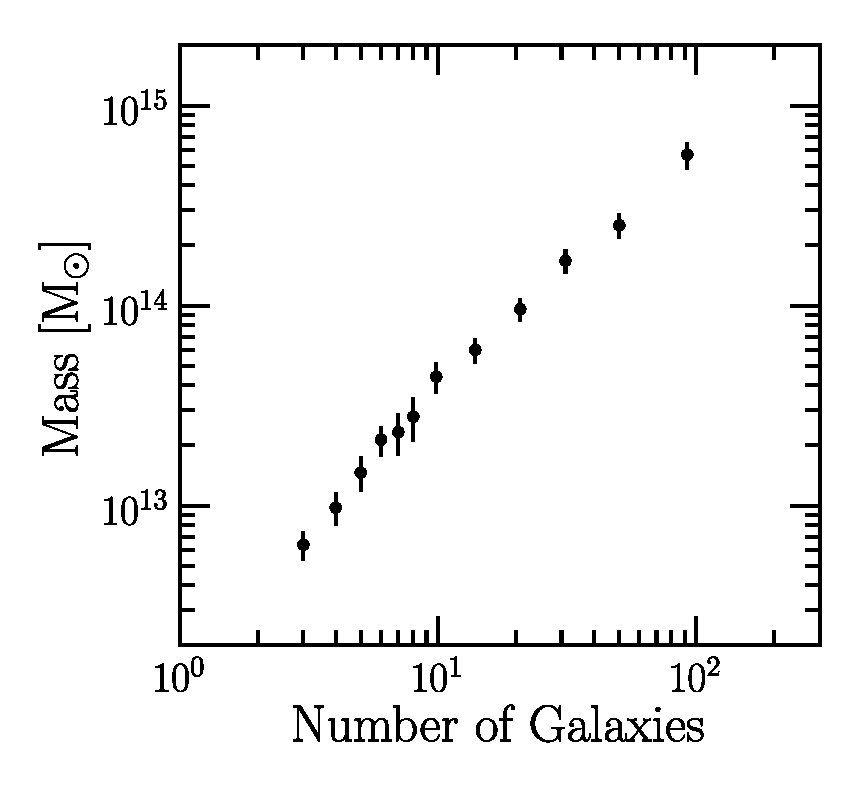
\includegraphics[scale=0.7]{mass-rich-plot.eps}
\caption{Mean mass as a function of the number of
galaxies in the group/cluster as measured by the PI from lensing in SDSS
data \cite{SheldonLensing07,JohnstonLensing07}. This calibration
is critical to measuring Dark Energy with galaxy clusters.\label{fig:massngals}}
\end{figure}




From measurements using galaxies as the lenses, we confirmed that there is an
enormous amount of unseen dark matter in galaxies, and that this dark matter is
in a ``dark halo'' that extends far beyond the concentrated bundle of stars at
the center of galaxies.  We have found similar results for groups and clusters
of galaxies; there is a pool of Dark Matter between galaxies in the group.
These measurements are completely consistent with the cold dark matter model.
A number of derived results have come from these basic measurement papers, in
which we have learned a great deal about the connection between the dark and
visible matter in galaxies and clusters, e.g.
\cite{RykoffLXM08,RozoScatter09,TinkerM2N2012}. 

Sheldon and collaborators have also used these measurements to estimate
cosmological parameters.  As stated in the introduction, the number density of
halos of a given mass is related to the mean mass density of the universe and
variance in the density.  In \cite{RozoCosmo09} we combined the counts of
galaxy clusters with our lensing mass estimates to constrain these cosmological
parameters.  Figure \ref{fig:omegasigma8} shows results from \cite{RozoCosmo09}
constraining the fractional mass density $\Omega_m$ (relative to the total
energy density) and the variance in mass density on 8 Mpc scales $\sigma_8$
relative to the mean. In \cite{TinkerM2N2012} we used the ratio of mass to
number density in clusters, combined with the large scale clustering of all
galaxies, to place further complementary constraints on $\Omega_m$ and
$\sigma_8$.  All these results are consistent with one another and the Cold
Dark Matter theory.

\begin{figure}[p] 
\centering 
\includegraphics[scale=0.6]{s8_Om.ps}

\caption{Constraints on the mass density of our universe $\Omega_m$ (relative
    to the total energy density) and the variance in the density on 8 Mpc
    scales $\sigma_8$, relative to the mean, as measured from SDSS data.  These
    results \cite{RozoCosmo09} are derived by combining the counts of galaxy
    clusters with the mass calibrations from gravitational lensing as shown in
    Figure \ref{fig:massngals} \cite{SheldonLensing07,JohnstonLensing07}.  The
    cluster results break degeneracies with other probes such as the cosmic
microwave background (WMAP).  With DES we will study Dark Energy properties by
extending these measurements back in time.  \label{fig:omegasigma8}} 

\end{figure}


While powerful in themselves, these results are also very complementary to
other measurements, breaking degeneracies in analyses of the Cosmic Microwave
Background \cite{KomatsuWMAPCosmo09}. 

Gravitational shear measurements are central to two of the primary goals of the
Dark Energy Survey (DES, section \ref{sec:des}).  The techniques we developed
in the SDSS are directly applicable to DES science, especially the study of
galaxy clusters as cosmological probes.  By extending the measurements backward
in time with the deeper DES data, we will learn about Dark Energy as well as
Dark Matter.


\subsection{The Dark Energy Survey (DES)} \label{sec:des}

The Dark Energy Survey (DES) is an optical, multi-band survey of 5000 square
degrees using the 4-meter ``Blanco'' telescope at the Cerro Tololo
Inter-American Observatory in Chile. A new camera is being built and the
telescope repaired and upgraded.  The DES will utilize gravitational lensing,
an optical cluster survey, supernovae, and galaxy clustering to constrain the
properties of Dark Energy.  Combining DES lensing measurements and DES optical
observations of galaxy clusters with observations by the South Pole Telescope
(SPT, \cite{SPT04}) of the same galaxy clusters, greatly enhances the
constraining power.  These combined methods will constrain the Dark Energy
equation of state parameter $w$ to better than 3\%; an important component of
this overall constraint will be the cluster lensing measurements led by
Sheldon.  First light occured in \commissdate, and the survey will run for five
years.  DES is funded in part by the U.S. Department of Energy. 


The SPT will use the Sunyaev-Zel'dovich (SZ) Effect \cite{Birkinshaw99}, the
Compton up-scattering of light from the cosmic microwave background by the hot
gas in galaxy clusters, to find a complete sample of clusters to high redshift.
This selection of this cluster sample is complementary to the DES optical
cluster selection in that it is expected to be nearly independent of the
distance of the cluster from the observer.  As with DES, the goal of the SPT is
to use these clusters to probe the growth of structure, and the volume of
space, as a function of time in order to constrain Dark Energy.  Since it is
the number density of clusters of a given mass that is sensitive to Dark
Energy, an important part of each cluster survey will be the calibration of the
mass-observable relationship via lensing.  In \S \ref{sec:deslensing} we will
describe in detail our plans for measuring this relationship using DES optical
data.

In addition to galaxy clusters, the DES will use a number of other probes to
constrain Dark Energy properties.  These include two other lensing probes:
Shear-shear correlations as a function of scale and the cross-correlation
between shear and known objects as a function of scale.  Data are shared
between cluster mass measurements and these probes, but because the correlation
functions cover a much larger range of scales, they are complementary.  There
is also a Supernova program that, while less constraining by itself, breaks
degeneracies between certain cosmological parameters.  

Table \ref{table:constraints} contains forcasted constraints on $w$ for various
techniques employed by DES \cite{DESWhitePaper}.  These forecasts are for DES
and SPT data alone; combining with other data, for example from cosmic
microwave background measurements from the Planck satellite
\cite{PlanckBluebook}, can significantly increase the precision of certain
probes.

\begin{deluxetable}{ll}
\tablecaption{Projected DES Constraints on Constant $w$ Dark Energy Models.
\label{table:constraints}}
\tablewidth{0pt}
\tablehead{
	\multicolumn{1}{l}{Method} &
	\colhead{$\sigma_w$}
}
\startdata
Clusters &  \\
~~~Abundance & 0.13  \\
~~~with WL Calibration & 0.09 \\
Weak Lensing & \\
~~~Cosmic Shear (CS) & 0.15  \\
~~~Galaxy/Cluster-shear(GS) + Angular Clustering(AC) & 0.08  \\
~~~CS + GS + AC & 0.03  \\
Angular Clustering of Galaxies & 0.36 \\
Supernovae Ia & 0.34 \\
\enddata
\end{deluxetable}

\subsection{DES Builder} \label{sec:builder}

Sheldon was awarded DES ``builder'' status for his service to the survey.
Sheldon initially began work on DES in 2004.  He worked to plan the survey,
studying various possible systematics informed by real data. He forecasted the
sensitivity of the DES to lensing effects under realistic observing conditions,
which ``flowed down'' to constraints for the camera/telescope system. This work
also informed the survey strategy, helping to optimize the spatial/temporal
observing pattern on the sky and in time to limit systematic effects for
lensing.  Sheldon has since worked on building software pipelines to process
DES images to measure lensing effects.  He has built a generic, pluggable image
processing framework; multiple lensing codes have been used in this framework
to process the realistic simulated DES images, including the new method
described in \ref{sec:gmix}.

\subsection{Overview of DES Activities}

The work on DES has two primary aspects of interest for this proposal:
development of techniques to measure gravitational shear and science analysis
of the shear in terms of Dark Energy.  Sheldon will focus primarily on
developing shear measurement techniques, including a promising new technique
and a fast implementation using graphics processing units.  Sheldon will guide
a research associate to analyze these measurements to extract cosmological
parameters.  In the following sections we will describe the current state of
this research and planned activities.

\subsection{Lensing Analysis of DES Data} \label{sec:deslensing}

\subsubsection{Science Analysis}

As described in the introduction, the cosmological information from clusters is
primarily in the number density of objects with a given mass as a function of
time, especially the most massive objects such as galaxy clusters.  Clusters
are identified not by their mass but by other indicators, such as the number of
galaxies in a cluster or the SZ effect.  The SZ effect and the number of
galaxies are both correlated with mass, but that correlation must be measured
by a secondary method.  As described in the introduction, lensing is the best
method for doing this.  

As described in \S\ref{sec:sdssold}, in our studies of SDSS lensing we
developed analysis techniques to calibrate the mass-observable relation of
clusters (Figure \ref{fig:massngals}).  Using this calibration in conjunction
with the number density we have inferred cosmological parameters (Figure
\ref{fig:omegasigma8}).  These techniques are limited only by our understanding
of the systematics and characterization of the cluster selection process.  The
volume and depth of DES is sufficiently large to perform measurements
equivalent to the SDSS study, but separately in many bins of cosmic time.  Time
dependent measurements will allow us to extend our cosmological analysis to
constrain the properties of Dark Energy.

There is much room for innovation in this field: the sensitivity of DES will be
such that small systematic effects will become important. Some such issues are:
offsets between the identified galaxy cluster position and the true center of
mass; measurements errors due to object overlap in crowded regions at cluster
centers; errors introduced by distance uncertainties in the cluster catalog and
source catalog; bias in the orientation of clusters introduced by the cluster
finding procedure.  At the same time, the great sensitivity of DES imaging will
create the potential to explore entirely new lensing-based probes.  What we
learn from DES, the largest survey to date, will be highly influential for
future surveys such as LSST. Note BNL is an LSST member institution, and
Sheldon will begin participating in LSST as DES finishes.

In contrast with cluster lensing measurements, the ``cosmic shear'' is the
correlation of shears across the sky independent of the location of foreground
structures.  Since the shear is related to mass, the cosmic shear can be used
to infer statistics of the underlying mass distribution, the evolution of which
is directly related to the properties of Dark Energy.  Because the signal need
not be modeled in terms of cluster halos, the interpretation of cosmic shear
can be simpler than cluster lensing.  However, the measurement involves
directly correlating shears from many sources as a function of their separation
on the sky, which can propagate systematic errors directly into the
measurement. Thus cosmic shear and cluster lensing are quite complementary.

Table \ref{table:constraints} contains a list of DES probes and their power to
constrain the equation of state $w$.  If the desired accuracy is achieved,
cluster lensing (clusters with weak lensing calibration), which is being led by
Sheldon, is the most sensitive probe.

Erin Sheldon will guide a research associate in using shear measurements to
calibrate the masses of the galaxy clusters used in the cosmological analyses.
We will also work with other DES collaborators on the measurement of cosmic
shear.  These are critical components of the DES mission.  We expect major
results to appear after year one based on the single epoch data, year 2-3 after
multi-epoch data becomes available, and at survey end with the final data set.

In our forecasting of cosmological parameter constraints, we have assumed we
can meet a certain level of lensing shear measurement accuracy.  This analysis
is ultimately limited by how accurately we can measure galaxy ellipticities and
remove the effects of the point spread function.  In the next section we will
address the second major part of this proposal: a new method to measure shear
and a fast implementation on graphics processing units.

\subsection{New Lensing Shear Measurement Technique Using Gaussian Mixtures}
\label{sec:gmix}

The weak gravitational shear effect discussed in the previous sections is a
very small distortion of the images of galaxies by foreground mass
distributions due to the bending of light.  This small distortion produces
correlations in the ellipticities of the background galaxies, which can only be
measured statistically.  In principle all one needs is enough galaxies to
extract this signal from the noise.  However, the telescope optics and
atmosphere distort and blur the images of galaxies, and this also produces
correlations in the ellipticities of galaxies; the combined effect is generally
referred to as the point spread function (PSF). The primary affect is a
convolution, which means the effect is more significant for smaller galaxies.
Most detected galaxies are of order the size of the PSF, and the effect is
typically at a level much larger than the lensing effect we wish to measure.

Many methods have been developed to measure and remove the effect of the PSF to
produce unbiased ellipticity measurements, e.g.
\cite{ksb95,Bern02,Miller07,Melchior11} and there are many more.  No method yet
tested has proven accurate enough to meet the DES survey requirements when
applied to realistic galaxy populations:  for DES to meet the projected
constraints on dark energy, the fractional error on the shear cannot exceed
0.004.

Erin Sheldon has developed a new technique that shows promise to meet the DES
requirements.  The method uses mixtures of Gaussians to represent the galaxies
and PSF, and bayesian techniques to control noise bias.  This model has enough
flexibility to represent the canonical galaxy types; this has recently been
independently verified \citep{HoggGMix12}.  One result of our recent research
is that many fewer Gaussians are required than used in \cite{HoggGMix12} when
the object is of order the size of the PSF; three is enough.  
%When also
%demanding the Gaussians are co-centric and co-elliptical the parameter space is
%reduced even further.  

It is tempting to just use the canonical galaxy profiles (exponential disks and
\devprof\ ``\devauc'' profiles) to fit for the ellipticity, but these are
computationally intensive to generate when convolving with a PSF and the pixel
response.  Using Gaussians for both PSF and galaxy greatly increases the speed
because the convolutions can be done analytically.   Furthermore, the Gaussian
mixture model can adapt to profiles that differ from the canonical models.

Other features of the method are more generic and are designed to mitigate the
effects of noise.  Noise is known to produce bias in the shear measurement when
using either maximum likelihood \cite{Refreg12} or the expectation value
derived from a full exploration of the likelihood \cite{Miller12}.  This can be
mitigated using the techniques in \cite{Miller07,Miller12}. These techniques
involve measuring the full likelihood surface and applying prior information on
the ellipticity distribution of the galaxy population as a whole\footnote{In
\cite{Miller12} a prior on size is applied, but we have found this unnecessary
if a proper \snsize\ cut is made}.
Corrections can then be derived to mitigate bias introduced by the priors and
noise.  Sheldon has implemented these techniques using a Monte Carlo Markov
Chain technique, and the code is publicly available (although the use of priors
is clearly described in \cite{Miller07}, that author's code is proprietary).

The results from simulations indicate the method can potentially meet DES
requirements.  The shear bias as a function of signal-to-noise ratio \snsize\
is shown in Figure \ref{fig:getgdt}.  Results for simulated exponential disk galaxies
are shown in the left panel.  Galaxies with \devprof\ profiles are shown in the
right panel.  The DES requirement is shown as the gray band.  The DES
requirements for shear accuracy are met for galaxies with \snsize\ $>$
\sncut.  

The value \snsize\ is the signal-to-noise ratio of the measured size
$T=\sigma^2$ of the object.  The \snsize\ is a good indicator because galaxies
with different profiles have similar shear bias at fixed \snsize.  In contrast,
the weighted S/N of the flux is not a good indicator: objects at fixed weighted
flux S/N have different shear bias.  This effect is not completely understood,
but it is true that size and ellipticity are degenerate in these fits, and a
very poorly constrained size results in more scatter in the ellipticity and
more noise bias.

\begin{figure}[t]
\centering

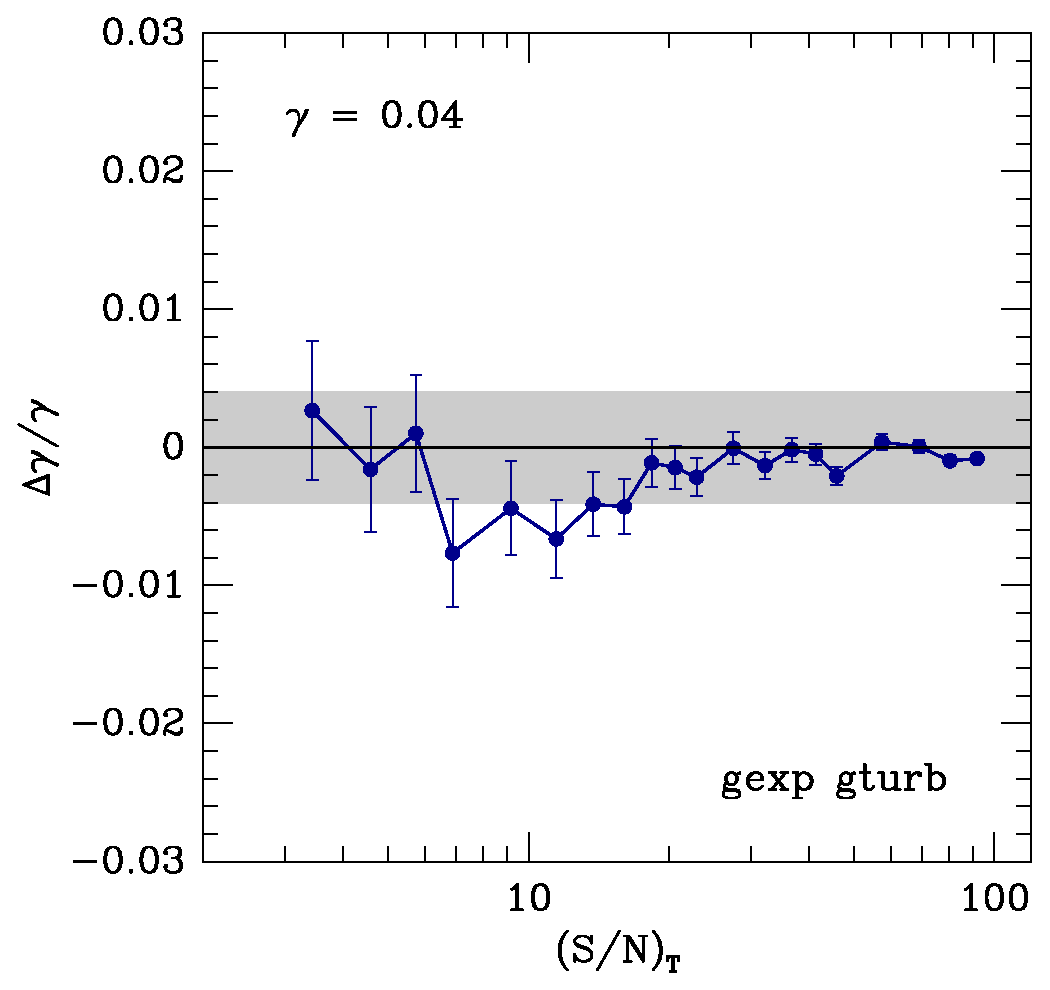
\includegraphics[scale=0.4]{mcbayes-get03r01r02r03r04r05-yr-0.030-0.030-frac.eps}
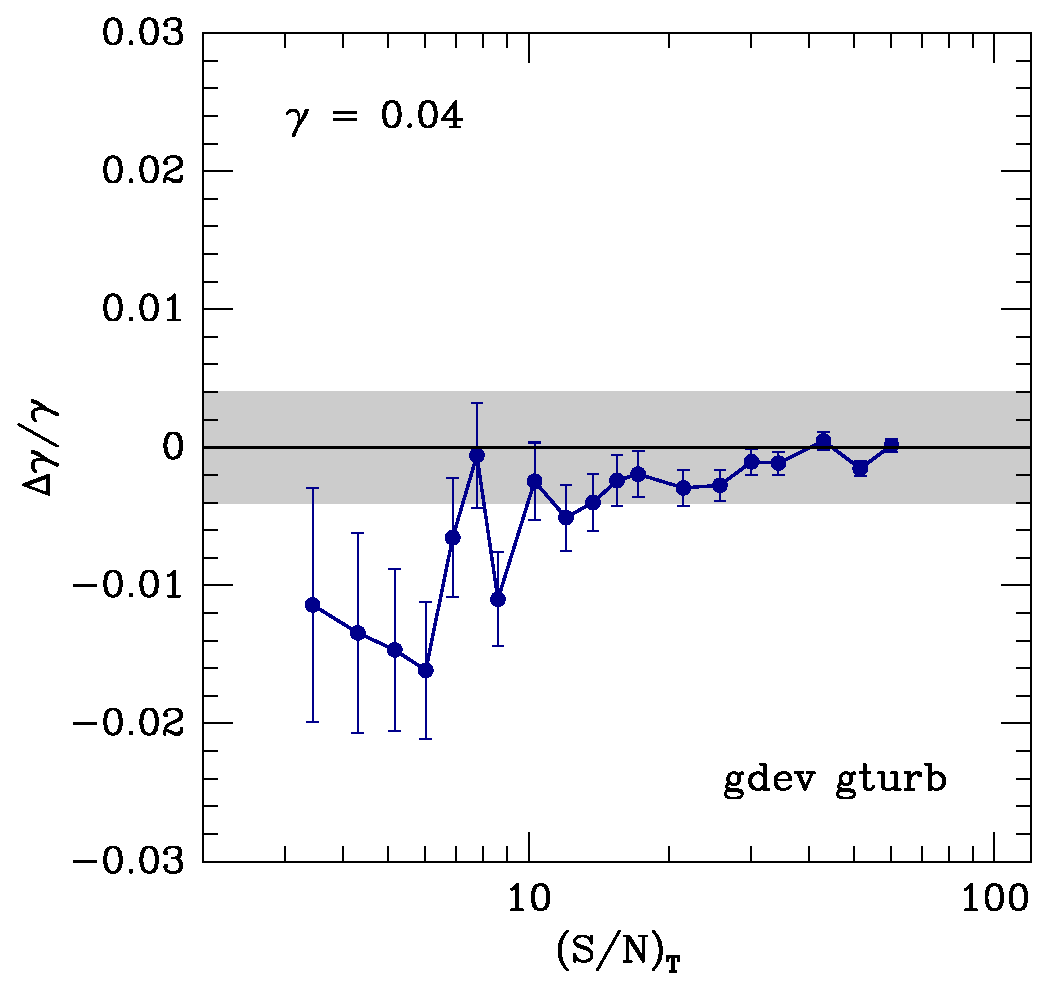
\includegraphics[scale=0.4]{mcbayes-gdt03r01r02r03r04-yr-0.030-0.030-frac.eps}

\caption{Fractional shear bias as a function of the signal-to-noise ratio
    \snsize\ of the object scale size.  The simulated galaxies are comparable
    in size to the PSF.  The PSF represents atmospheric turbulence.  Left
    panel: Simulated exponential disk galaxies fit by a Gaussian mixture.  A
    prior on the distribution of ellipticities has been applied.  The gray band
    is the DES requirement on the shear bias. Right panel: Same as the left
    panel but for simulated \devprof\ galaxies.  These simulations indicate a
    cut on \snsize\ $>$ \sncut\ removes the most biased sample.
\label{fig:getgdt} }

\end{figure}

\subsubsection{Speeding Up the Computations with GPUs} \label{sec:gmix:gpu}

The corrections discussed in the previous section require measurement of the
full likelihood surface, and are thus very computationally intensive.  Using
the Gaussian mixture provides fast convolutions, but the large number of
likelihood evaluations requires of order 2 seconds per galaxy on a CPU (2.7 GHz
intel). The requirements to process the full DES will be enormous: the expected
500 million galaxies will be observed on $\sim$ 10 separate exposures, which
would require $\sim$ 3 million cpu hours to process. Note the CPU computation
is highly optimized, including a fast approximate exponential function five
times faster than the standard. 

We have found significant gains in speed by using a graphics processing unit
(GPU).  This problem is particularly suited to GPU processing because the image
must be uploaded only once, and then thousands of likelihood evaluations are
made on the GPU. Only a single number, the likelihood, must be returned by the
calculations, minimizing the overhead of moving data back and forth from the
GPU memory.  We have found that each likelihood calculation is faster by a
factor of $>$\speedupnum\ compared to the CPU code, primarily due to
parallelization of the pixel rendering of the model; each pixel can be rendered
in parallel.

Further speedup was obtained by parallelizing the Markov chain.  We use an
affine invariant Markov chain\cite{GoodmanWeare10} with twenty separate
``walkers'' that are evaluated independently at each step.  The total speedup
is about a factor of \overallspeedup.  This is somewhat less than the 20x10=200
possible speedup due to data transfer overhead.  This gain of \overallspeedup\
is due to the extreme parallelization possible with this problem.  This
parallelization is made possible by the small image dimensions for a typical
galaxy (25x25) and independence of the likelihood evaluations for each walker
at a given step.

We can also make use of multiple GPUs attached to a single machine; we shall
propose attaching \ngpus.  Of cource there are also typically multiple CPUs per
system.  Comparing a \ngpus\ GPU system to a \ncpus-core CPU system, the total
speedup is \ngpus*\overallspeedup/\ncpus = \speedupcpu.

These increases in speed come at a moderate increase in cost over typical
``farm'' compute nodes.  Adding \ngpus\ high performance GPUs to a typical node
increases the cost by about a factor or \costincrease. In section
\ref{sec:computing} we will outline the moderate cost to build a sufficient set
of machines to process the DES data.

{\it
    
Notes:  All the code was written in the C language with OpenCL extensions by
Erin Sheldon and is publicly available.  Using OpenCL means we are not tied to
any vendor-specific optimizations and could in principle use GPUs from vendors
other than Nvidia. Some more time can be spent tuning the GPU implementation.
On the other hand, the ultimate bottleneck will be memory bandwidth
limitations, which these tests may already have met.   More walkers could be
used for better parallelization, but the tradeoff is a more costly burn-in for
the Markov chain, as the total burn-in does not decrease inversely with the
number walkers.  A ``high-end'' graphics card is required to get this speedup;
we tested an Nvidia 2050. The comparison CPUs are 2.7 GHz intel Xeon
processors.  The number of likelihood evaluations needed is the number of
walkers times (burn-in + steps).  For higher S/N objects, a burn-in of about
400 steps per walker is needed, followed by 200 steps.  A large number is
needed after burn-in to measure the tails of the distribution, which are
important.  A high performance distributed file system is needed to get the
required data throughput: the cosmology group at BNL uses the Hadoop
Distributed File System, which provides sufficient throughput by allowing jobs
to run on the same machine holding the data; input/output from disk is only
about \iooverhead\ overhead.  }

\subsubsection{Future Work on Gaussian Mixtures}

There is much future work to be done on the Gaussian Mixture method.  We must
determine the priors on the ellipticity distribution from real data.  This is a
topic of research because, at faint magnitudes, it is difficult to determine
these distributions, especially for \devprof\ galaxies\cite{Miller12}.  Another
area of focus will be testing the method on more complex simulated galaxy and
PSF models.  Finally, the ultimate test is real data and we expect getting the
method to work optimally on real data will require the most effort.


\begin{comment}
\subsection{Shear Measurement Using Shapelets}
\label{sec:shapelets}

In addition to the Gaussian mixture method described in section \ref{sec:gmix},
Mike Jarvis of the University of Pennsylvania and I have implemented a full
shear pipeline based on the shapelets technique\cite{Bern02}.   The accuracy
does not yet meet DES requirements, but this pipeline is mature in the sense
that it can now run fully autonomously on the data and is fast and stable.
Tuning of the pipeline to increase accuracy is being led by Jarvis and is
showing promise.   The ideas for reducing bias, outlined in section
\ref{sec:gmix}, can in principle be applied to this technique as well.

This pipeline can make full use of the multi-epoch DES data where the sky is
observed many times.  This code has been tested on simulated DES data and will
continue to undergo heavy testing and refinement throughout the commissioning
phase.  

The processing framework was implemented by Sheldon.  This framework is
``pluggable'' so that other codes can be plugged in readily and can make use of
the infrastructure built around the shapelets code.  I plan to plug in the
Gaussian mixture code as well as 2-3 other pipelines developed within DES.

Note the shapelets pipeline, as it is implemented currently, gains less from a
GPU implementation than the Gaussian mixtures because it is a maximum
likelihood technique and so requires relatively few evaluations.  That said,
significant gains should be possible.  And, if the bias-correction schemes
discussed in section \ref{sec:gmix} are implemented for shapelets, then greater
gains can be had using GPUs.
\end{comment}

\subsection{Personnel and Resources} \label{sec:resources}

\subsubsection{Research Associate}

This grant will be used to fund our current postdoc, Andres Plazas, for the
first two years of the award. Plazas is already working on DES and it makes
sense for him to continue under this funding.  A second postdoc will begin in
the third year after Plazas' departure.  

The work of these postdocs will focus on high-level science analysis.  In
particular, we have carved out a niche in the field of cluster lensing and
cosmology, and we expect the postdocs will primarily work on that analysis.  As
outlined in section \ref{sec:sdssold}, this involves interpreting the shear in
terms of mass, and incorporating this into an overall measurement of cosmology.
These analyses will be important and will have high scientific impact, as
cluster lensing and cosmology is one of the primary probes used in DES.

Other analyses are also available at the postdocs discretion; the DES data set
will present an opportunity to explore new lensing-based probes.  Postdocs well
versed in computation may help with the computationally intense, GPU-based,
Gaussian Mixture technique outlined in section \ref{sec:gmix}.

\subsubsection{Computing} \label{sec:computing}

In section \ref{sec:gmix} we described a promising new shear measurement
technique based on Gaussian mixtures, and a fast implementation on graphics
processing units (GPUs).  Here we will give justification for funding a
moderate computing purchase with this grant.

We will have a lot of data to process.  We are commissioning the DES survey at
the time of this writing (\commissdate) and will run for five years, generating
about a petabyte of data in total.  For lensing we will process all the reduced
images, including analysis of multiple epochs for each pointing.  This subset
represents about 130TB of data.

The NSF funded Dark Energy Survey data management team will process the data
using a selected lensing pipeline approximately yearly.  However, the Gaussian
mixture pipeline is still in heavy development and will require many runs on
the data and simulations to find and fix bugs.  A turnaround time more like
$\sim$2.5 weeks on the full data set is desirable.   This will facilitate
development in response to data-driven needs as well as provide sufficient
computing for any simulation tests we require.

%Note the DES collaboration may also have some computing available to run the
%pipelines, but these systems will not be GPU based so the computationally
%intensive Gaussian mixture code is not a good use of that resource.

As described in section \ref{sec:gmix:gpu}, we want to process all 500 million
galaxies, each on 10 separate exposures, in this time of 2.5 weeks. Time per
galaxy is about 1.75 seconds on a 2.7GHz Intel CPU. In section
\ref{sec:gmix:gpu}, we showed this time can be reduced to 0.01 seconds using a
Nvidia 205 GPU.  Input output from a local disk (which we can guarantee using
the file system described in section \ref{sec:gmix:gpu}), is about \iooverhead\
overhead.  Thus we would require only $\sim$ \nmachines\ nodes with \ngpus\
GPUs each to process the survey in 2.5 weeks. 
%We round this up to 10 nodes for two reasons: 1) the Gaussian mixture
%algorithm is under development and computational requirements may increase and
%2) it is more cost-effective and efficient for data throughput to spread the
%required disk to more machines.  

What type of systems should these be?  We desire fairly large memory on the
system in order to hold data from all exposures in memory for a full ``coadd
tile''. A coadd tile is the unit of association used when combining exposures
and covers several tens of pointings, (with about ten exposures per pointing).
Tests indicate 32GB is sufficient, but we prefer 48GB as this is a better
number per core and is not a large increase in cost.  We need 130TB in the
distributed file system, so $\sim$ \diskper\ per machine(we are doing without
redundancy as the data are readily available for download from the DES
collaboration).  Recent purchases for the Atlas experiment at BNL are very
similar to this and we project a cost of approximately \basecost.  The addition
of \ngpus\ high-performance GPUs (e.g.  Nvidia 2050) adds another $\sim$
\costgpu. Note we could increase the number of GPUs per machine and buy fewer
machines but we would then have difficulty getting the required amount of disk
on the machines at a reasonable cost.  The total cost is about \totalcost.
Note overhead is also included in the budget, but not escalation as we expect
the machines to become somewhat cheaper at fixed performance.  These can be
purchased over the five year survey.  There is potential for increase in speed
per GPU, but this is difficult to predict currently as scientific GPUs are a
new technology.  We prefer to quote the current performance profile.

Note these prices include bulk discounts from purchasing along with other
experiments through the RHIC-Atlas Computing Facility at BNL.  

\begin{deluxetable}{lcc}
    \tabletypesize{\small}
    \tablecaption{Projected Computing Purchases\label{table:computing}}
    \tablewidth{0pt}
    \tablehead{
        \multicolumn{1}{l}{Fiscal Year} &
        \colhead{Compute Servers with 2 GPUs}   & 
        \colhead{Total Storage} \\
        &
        &
        [TB]
    }
    \startdata
2013 & 2 & 26 \\
2014 & 2 & 26 \\
2015 & 2 & 26 \\
2016 & 2 & 26 \\
2017 & 2 & 26 \\
\hline
\relax\\[-1.7ex]
Total in 5 years & 10 & 130 TB \\\\[-2.7ex]
\enddata

    \tablecomments{The number of compute nodes purchased is based on the
    assumption that each node and GPU (Intel 12 cores, 32GB ram, two nvidia
    2050 GPUS) would stay at the performance level of a node purchased in 2012.
    It is not clear how the performance per GPU will increase over time so this
    table is conservative.  Disk is likely to get cheaper, so the 13TB per
    machine could be expanded at fixed cost. Power, cooling and maintenance
    will be provided at no extra cost to this experiment, but overhead 
    and slight escalation are included in the budget.}

    \end{deluxetable}
    


\subsubsection{Salary and Travel}

It is required that DOE employees pay their salary from this grant, so 100\% of
Erin Sheldon's salary and overhead for five years is requested.  We also request
support for a research associate for five years.

The remaining expenses beyond salary and computing are primarily for travel.
Erin Sheldon and a postdoc will travel to a DES collaboration meeting each
year.  Sheldon plans to spend three weeks each summer at a workshop in the US,
such as those held at Aspen and Santa Fe.  Further travel will involve
attending a few conferences per year across the US for both Sheldon and
postdoc.  Erin Sheldon will also make regular trips to the University of
Pennsylvania to collaborate with fellow DES weak lensers Mike Jarvis and
Bhuvnesh Jain.

\clearpage
\newpage
\subsection{Timeline} \label{sec:timeline}

This is an outline of the activities for the five year extent of the award.
For reasons of continuity, we will begin the timeline in Fall 2012.  It is
assumed that the primary collaborators on these activities are Erin Sheldon of
BNL and a postdoc, or research associate.

\begin{itemize}

\item {\bf Fall 2012-Spring 2013} Process and evaluate commissioning data as it
    arrives.  Continued testing of the weak lensing pipelines on simulated
    data.

\item {\bf Late Spring through end of 2013} Survey proper begins; process data
    as it arrives.  Re-process data as bugs are found and algorithms improve.
    Processing using Gaussian mixtures at BNL on GPU cluster.  Begin science
    lensing analysis.

\item {\bf 2014} Continue processing data and testing pipelines.  Publication
    of first year DES measurements for galaxy and cluster-mass correlations.

\item {\bf 2015} Continue processing data as it arrives.  Continue improving
    algorithms.   First publications using multi-epoch data in 2014.

\item {\bf 2016-2017}  Activities should continue as before until survey end.
    Processing data as it arrives, incrementally improving the data pipelines
    and analysis codes.  Analysis methods will evolve, especially as the final
    data are in hand and there are many epochs with which to work.   There will
    be intermediate publications based on this data.

\item {\bf Post survey} A re-processing of all data through the final pipelines
    and final analysis of the full dataset to extract cosmological information.


\end{itemize}







\newpage
\addcontentsline{toc}{section}{Appendix 1: Biographical Sketch}
\section*{Appendix 1: Biographical Sketch}

%\setlength{\oddsidemargin}{-0.1in}
%\setlength{\evensidemargin}{-0.1in}
%\setlength{\textwidth}{6.7in}
%\setlength{\topmargin}{-0.25in}
%\setlength{\textheight}{9.0in}

\newcommand{\tsp}{\vspace{0.1cm}}
\newcommand{\isp}{\vspace{0.3cm}}
\newcommand{\ssp}{\vspace{0.4cm}}


{\Large {\bf Erin Sheldon}}
\tsp
%
% Address information.
%

\noindent
Bldg 510

\noindent
Brookhaven National Laboratory

\noindent
Upton, NY 11973

\noindent
(631) 344-3117

\noindent
erin.sheldon@gmail.com

\newcommand{\myshorttab}{0.5in}
\newcommand{\mytab}{0.75in}
\newcommand{\mylongtab}{1.25in}

\vspace{0.4cm}
\noindent
\makebox[1.25in][l]{{\large \bf Education and Training}}{}
\vspace{0.2cm}
\newline
\makebox[\mytab][l]{}{Postdoctoral Fellow, Center for Cosmology and Particle Physics}
\newline
\makebox[\mylongtab][l]{}{~~~~~~~~~~~~~~~~~~~~~~~~~~~~~{\bf New York University}}
    \hfill
    \makebox[1in][r]{{\small \it Sep 2005--Sep 2008}}
\newline
\makebox[\mytab][l]{}{Postdoctoral Fellow, Kavli Institute for Cosmological Physics}
	\newline
\makebox[\mylongtab][l]{}{~~~~~~~~~~~~~~~~~~~~~~~~~~~~~{\bf University of Chicago}}
	\hfill
	\makebox[1in][r]{{\small \it Aug 2002--Aug 2005}}
\newline
\makebox[\mytab][l]{}{Research Assistant, {\bf FNAL}}
	\hfill
	\makebox[1in][r]{\small \it Jun 1998--Sep 1998}
\newline
\tsp
\noindent
\makebox[\mytab][l]{}{Ph.D., {\bf University of Michigan}}
    \hfill
    \makebox[1in][r]{\small \it Sep 1997--Aug 2002}
\newline
\tsp
\makebox[\mytab][l]{}{B.S., {\bf University of Missouri}}
\hfill
\makebox[1in][r]{\small \it Aug 1992 -- May 1997}


%
% Experience...
%

\vspace{0.4cm}
\noindent
\makebox[1.25in][l]{{\large \bf Experience}}{}
\newline
\vspace{0.2cm}
\makebox[\mytab][l]{}{Physicist, {\bf Brookhaven National Laboratory}}
\newline
\makebox[1.25in][l]{}{}
        \hfill
        \makebox[1in][r]{{\small \it Jan 2012--present}}
\newline
\vspace{0.2cm}
\makebox[\mytab][l]{}{Associate Physicist, {\bf Brookhaven National Laboratory}}
\newline
\makebox[1.25in][l]{}{}
        \hfill
        \makebox[1in][r]{{\small \it 2010--2012}}
\newline
\vspace{0.2cm}
\makebox[\mytab][l]{}{Assistant Physicist, {\bf Brookhaven National Laboratory}}
\newline
\makebox[1.25in][l]{}{}
        \hfill
        \makebox[1in][r]{{\small \it Sep 2008--2010}}




\vspace{0.3cm}
\noindent
\makebox[1.25in][l]{{\large \bf Graduate and Postdoctoral Advisors and Advisees}}{}
\vspace{0.2cm}
\newline
\makebox[\myshorttab][l]{}{{\large \bf Advisors}}
\newline
\makebox[\mytab][l]{}{Postdoctoral Advisor: David Hogg, New York University}
\newline
\makebox[\mytab][l]{}{Postdoctoral Advisor: Josh Frieman, University of Chicago}
\newline
\makebox[\mytab][l]{}{Thesis Advisor: Timothy McKay, University of Michigan}
\newline
\makebox[\myshorttab][l]{}{{\large \bf Advisees}}
\newline
\makebox[\mytab][l]{}{Postdoc, BNL: Zhaoming Ma}
\newline
\makebox[\mytab][l]{}{Postdoc, BNL: Andres Plazas}


%\noindent
%\makebox[1.25in][l]{}
%\parbox{5.40in}{
%Ph.D., Physics\newline
%Thesis advisor: Prof. Timothy McKay\newline
%Title of thesis: ``Galaxies, Luminosity, and Mass: Gravitational Lensing Measurements of the Correlation between Dark and Luminous Matter''
%}




\newpage
\vspace{0.2in}
\noindent
\newline
\newline
{\Large {\bf Selected Publications for Erin Sheldon} }
\newline
Note Appendix 3 holds the references for the narrative. 
\vspace{4mm}

\begin{tabular}{p{3mm} p{5.5in}}

1 & E.~S. {Sheldon} et~al.
\newblock {Photometric Redshift Probability Distributions for Galaxies in the SDSS DR8}.
\newblock {\em \apjs}, 201 32, August 2012. \\[6pt]

2 & J. {Tinker}, E.~S. {Sheldon} et~al.
\newblock {Cosmological Constraints from Galaxy Clustering and the Mass-to-Number Ratio of Galaxy Clusters}.
\newblock {\em \apj},  745:16 January 2012. \\[6pt]

3 & E. {Rozo} et~al.
\newblock {Cosmological Constraints from the Sloan Digital Sky Survey maxBCG Cluster Catalog}.
\newblock {\em \apj}, 708:645-660, January 2010. \\[6pt]

4 & E.~S. {Sheldon} et~al.
\newblock {Cross-correlation Weak Lensing of SDSS Galaxy Clusters III:
  Mass-to-light Ratios}.
\newblock {\em \apj}, 703:2232-2248, October 2009. \\[6pt]

5 & D.~E. {Johnston}, E.~S. {Sheldon}, et~al.
\newblock {Cross-correlation Weak Lensing of SDSS Galaxy Clusters II: Cluster
  Density Profiles and the Mass--Richness Relation}.
\newblock {\em arXiv:0709.1159}, September 2007. \\[6pt]

6 & E.~S. {Sheldon} et~al.
\newblock {Cross-correlation Weak Lensing of SDSS Galaxy Clusters I:
  Measurements}.
\newblock {\em \apj}, 703:2217-2231, October 2009. \\[6pt]

%5 & B.~P. {Koester} et~al.
%\newblock {A MaxBCG Catalog of 13,823 Galaxy Clusters from the Sloan Digital
%  Sky Survey}.
%\newblock {\em \apj}, 660:239--255, May 2007.\\[6pt]

7 & E.~S. {Sheldon} et~al.
\newblock {The Galaxy-Mass Correlation Function Measured from Weak Lensing in
  the Sloan Digital Sky Survey}.
\newblock {\em \aj}, 127:2544--2564, May 2004.\\[6pt]

%7 & T.~A. {McKay}, E.~S. {Sheldon}, D.~{Johnston}, E.~K. {Grebel}, F.~{Prada},
%  H.-W. {Rix}, N.~A. {Bahcall}, J.~{Brinkmann}, I.~{Csabai}, M.~{Fukugita},
%  D.~Q. {Lamb}, and D.~G. {York}.
%\newblock {Dynamical Confirmation of Sloan Digital Sky Survey Weak-lensing
%  Scaling Laws}.
%\newblock {\em \apjl}, 571:L85--L88, June 2002.\\[6pt]

8 & T.~A. {McKay}, E.~S. {Sheldon}, et~al.
\newblock {Galaxy Mass and Luminosity Scaling Laws Determined by Weak
  Gravitational Lensing}.
\newblock {\em ArXiv Astrophysics e-prints}, August 2001.\\[6pt]

9 & E.~S. {Sheldon} et~al.
\newblock {Weak-Lensing Measurements of 42 SDSS/RASS Galaxy Clusters}.
\newblock {\em \apj}, 554:881--887, June 2001.\\[6pt]

10 & P.~{Fischer}, T.~A. Mckay, E.~S. Sheldon, et~al.
\newblock {Weak Lensing with Sloan Digital Sky Survey Commissioning Data: The
  Galaxy-Mass Correlation Function to 1 Mpc}.
\newblock {\em \aj}, 120:1198--1208, September 2000.

\end{tabular}

\ssp
\ssp
\noindent
\parbox[l]{1.25in}{{\bf Synergistic \\ Activities}}
\parbox[t]{5.40in}{
Elected {\bf Builder} of the Dark Energy Survey {\it see section \ref{sec:builder}} \hfill {\small 2011} \newline
Elected {\bf Architect} of the Sloan Digital Sky Survey III \hfill {\small 2011} \newline
{\it For coordinating target selection, similar to DES builder} \newline
Reviewer for the Astrophysical Journal and Monthly Notices of the Royal Astronomical Society.
 \hfill {\small 2000-12}
}

\newpage

\vspace{0.2in}
\noindent
\newline
\newline
{\Large {\bf Selected Collaborators} }
\newline

\noindent
Blanton, Michael, New York University \newline
Cunha, Carlos, University of Michigan \newline
Dawson, Kyle, University of Utah \newline
Hogg, David, New York University \newline
Ho, Shirley, University of Pittsburgh \newline
Mandelbaum, Rachel,  Carnegie Mellon University \newline
McDonald, Pat, Brookhaven National Laboratory \newline
Myers, Adam, University of Wyoming \newline
Rozo, Eduardo, Kavli Institute for Cosmological Physics \newline
Schlegel, David, Lawrence Berkeley National Laboratory \newline
Slosar, Anze, Brookhaven National Laboratory \newline
Tinker, Jeremy, New York University \newline
Wechsler, Risa, Stanford University \newline
Weinberg, David, Ohio State University \newline
White, Martin, University of California-Berkeley \newline
Zehavi, Idit, Case Western Reserve University \newline



\newpage
\addcontentsline{toc}{section}{Appendix 2: Current and Pending Support}
\section*{Appendix 2: Current and Pending Support}

Dr. Erin S. Sheldon is currently supported for the 2012-2013 as a physicist at
Brookhaven National Laboratory at 100\%.   There is no other support pending;
i.e. there is currently no support for Sheldon for the period covered by this
proposal.  Pending project approval, support will come from this grant {\bf as
required for laboratory employeees}.

\vspace{5mm}
\noindent
Investigator: Erin Sheldon\newline
Source of Support: DOE Office of Science\newline
High Energy Physics\newline
FWP: PO104\newline
Period Covered: 10/1/12-9/30/13\newline
Man Months: 12 months

\begin{comment}
\begin{table}[h]
\begin{center}
\begin{tabular*}{0.85\textwidth}{ll}
B\&R \#YN010000  & \parbox[t]{\textwidth}{BNL Laboratory Directed 
   Research \& Development \\ Award} \\
                 & LDRD 10-45 (FY 2010 -– FY 2012) \\
                 & Astrophysics \& Cosmology Initiative \\
                 & 100\%
\end{tabular*}
\parbox{0.85\textwidth}{\caption{{\bf Current Funding}: Program Development 
\& Lab Directed Research \& Development \label{table:support}}}
\end{center}
\end{table}
\end{comment}


\newpage
\addcontentsline{toc}{section}{Appendix 3: Bibliography for Narrative}
\renewcommand{\refname}{\section*{Appendix 3: Bibliography for Narrative}\label{app:bib}}
\bibliographystyle{unsrt}
\bibliography{astroref}
\vspace{5mm}
\noindent
{\bf Key:} {\it AJ} is The Astronomical Journal, {\it ApJ} is The 
Astrophysical Journal and {\it MNRAS} is The Monthly Notices of the Royal
Astronomical Society.






\newpage
\addcontentsline{toc}{section}{Appendix 4: Facilities and Other Resources}
\section*{Appendix 4: Facilities and Other Resources}

We plan to acquire a moderate amount of computing.  The housing, power and
cooling, administration, and maintenance for these computers will be provided
by the RHIC-Atlas Computing Facility at Brookhaven National Lab at no
additional cost to this experiment.	The tests we performed on GPUs occured on a
machine in the RACF set aside for prototyping.  The engineers who set up this
system can lend expertise to tuning the new GPU systems purchased with this
grant.

\newpage
\addcontentsline{toc}{section}{Appendix 5: Equipment}
\section*{Appendix 5: Equipment}

The equipment {\bf currently} available to this project is shared time on a set
of 34 compute nodes and a file server purchased in 2009-2012.  
%The file server holds 40 TB. Nine of the compute nodes are 12 core with 32GB
%ram, twelve are 12 core with 48GB ram, and the rest are 8 core 32GB ram
%systems.  These are housed at the RHIC-Atlas Computing Facility at BNL.  
Because these are a highly over-subscribed, shared resource, only a fraction of
the resources can be dedicated to this project.  For this reason, we have requested
a moderate amount of computing to facilitate the proposed research, as outlined
in section \ref{sec:computing}

% this is a pdf insert
\newpage
\addcontentsline{toc}{section}{Appendix 6: Other Attachments}
fake for letter

\end{document}
